\documentclass{amsart}
\usepackage{amsmath, amssymb}
\usepackage{tikz-cd}
\usepackage{mathbbol} % mathbb on greek letters

% hyperref
\usepackage[bookmarks=true, linktocpage=true,
bookmarksnumbered=true, breaklinks=true,
pdfstartview=FitH, hyperfigures=false,
plainpages=false, naturalnames=true,
colorlinks=true, pagebackref=true,
pdfpagelabels]{hyperref}
\hypersetup{
	colorlinks,
	citecolor=blue,
	filecolor=blue,
	linkcolor=blue,
	urlcolor=blue
}

% layout
\setlength{\textwidth}{\paperwidth}
\addtolength{\textwidth}{-1.85in}
\setlength{\textheight}{\paperheight}
\addtolength{\textheight}{-2in}
\calclayout

% Updating to MSC2020
\makeatletter
\@namedef{subjclassname@2020}{%
	\textup{2020} Mathematics Subject Classification}
\makeatother

% elements
\renewcommand{\P}{\mathcal{P}}
\renewcommand{\S}{\mathbb{S}}
\newcommand{\A}{\mathcal{A}ssoc}
\newcommand{\M}{\mathcal{M}}

% sets
\newcommand{\Z}{\mathbb{Z}}
\newcommand{\id}{\mathrm{id}}
\newcommand{\End}{\mathrm{End}}
\newcommand{\Hom}{\mathrm{Hom}}
\newcommand{\Bij}{\mathfrak{Bij}}
\newcommand{\G}{\mathfrak{G}}

% categories
\newcommand{\Ch}{\mathsf{Mod}_R}
\newcommand{\Alg}{\mathsf{Alg}}
\newcommand{\coAlg}{\mathsf{coAlg}}
\newcommand{\sSet}{\mathsf{sSet}}
\newcommand{\cSet}{\mathsf{cSet}}
\newcommand{\Set}{\mathsf{Set}}
\newcommand{\Nec}{\mathsf{Nec}}
\newcommand{\nSet}{\mathsf{nSet}}
\newcommand{\Mon}{\mathsf{Mon}}

% functors
\DeclareMathOperator*{\tensor}{\otimes}
\newcommand{\chains}{N_\bullet}
\newcommand{\cochains}{N_\bullet}
\newcommand{\Uleft}{U_{left}}
\newcommand{\Uright}{U_{right}}
\newcommand{\op}{\mathrm{op}}
\DeclareMathOperator*{\colim}{colim}
\newcommand{\cobar}{\Omega}
\newcommand{\gcobar}{\mathbb{\Omega}}

% environments
\newtheorem{theorem}{Theorem}
\newtheorem{proposition}[theorem]{Proposition}
\theoremstyle{definition}
\newtheorem{definition}[theorem]{Definition}
\newtheorem{remark}[theorem]{Remark}
% comments
\newcommand{\anibal}[1]{\textcolor{blue}{#1}}

% drawings
\include{figures}

\begin{document}
\title{The cobar constructions as an $E_\infty$ Hopf algebra}
\author{Anibal M. Medina-Mardones}
\address{Max Plank Institute for Mathematics, Bonn, Germany}
\email{ammedmar@mpim-bonn.mpg.de}
\address{Department of Mathematics, University of Notre Dame, Notre Dame, IN, USA}
\email{amedinam@nd.edu}
\author{Your name}
\address{Your address}
\email{Your email}

\keywords{.}
\subjclass[2020]{.}

\begin{abstract}
	
\end{abstract} 

\vspace*{-1cm}

\maketitle

\tableofcontents

% !TEX root = ../cobar1.tex

\section{Introduction}

For any topological space $\fX$, its complex of simplicial or cubical singular chains $\Schains(\fX)$ -- regarded as a differential graded (dg) abelian group -- encodes the homology of $\fX$ in its quasi-isomorphism type.
More homotopical information can be stored in the quasi-isomorphism type of this chain complex if considered as a (dg) coassociative coalgebra, which we will denote $\SchainsA(\fX)$, where the coproduct comes from a canonical choice of chain approximation to the diagonal $\fX \to \fX \times \fX$.
%, attributed respectively to Alexander--Whitney and Serre.
For instance, the cohomology ring of $\fX$ is retained, but the action of the Steenrod algebra on its mod $p$ cohomology is not.

In Mandell's seminal work \cite{mandell2006homotopy_type} it is shown that, when $\fX$ is nilpotent and finite type, the entire homotopy type of $\fX$ can be encoded in the quasi-isomorphism type of this complex if considered as an $E_\infty$-coalgebra, a structure providing $\SchainsA(\fX)$ with coherent homotopies witnessing the derived cocommutativity of the coproduct coming from the strict symmetry of the diagonal map.

%In this work we are interested in modeling algebraically the homotopy type of the based loop space $\loops_x \fX$ of a pointed space $(\fX, x)$.
%Via concatenation of loops this space is a topological monoid, whose induced structure on the set of path-connected components is a group; the fundamental group of the underlying space.

The first contribution of this paper is to explicitly endow the cubical singular chains of the based loop space $\loops_x \fX$, with the structure of a monoidal $E_\infty$-coalgebra extending the Serre diagonal.
More specifically, we verify that the monoid structure induced on $\cSchains(\loops_x \fX)$ by the concatenation of loops is compatible with a natural $E_\infty$-coalgebra structure on cubical singular chains, similar to the one defined in \cite{medina2022cube_einfty}.
%We denote this functor by $\cchainsUM \colon \cSet \to \coAlg_\UM$

%We will also concern ourselves with another algebraic model approximating the homotopy type of $\loops_x \fX$.
%which was introduced by Adams \cite{adams1956cobar}.
%This model \cite{adams1956cobar} is obtained by applying Adams' celebrated \textit{cobar construction} functor $\cobar$ to a pointed version of the coalgebra of simplicial singular chains of $(\fX, x)$.
%The cobar functor may be thought of as an algebraic counterpart to the based loop space.
%Just like the based loop space functor is part of a duality between pointed topological spaces and group-like topological monoids, the cobar functor is part of one between a pointed version of dg coalgebras and monoids in chain complexes.
% (i.e. dg algebras).
%Adams' cobar construction provides a model for the quasi-isomorphism type of the monoid of chains on the based loop space.

Applying Adams' cobar construction to the coalgebra of simplicial singular chains of $(\fX, x)$, he obtained another monoidal algebraic model $\cobar \sSchainsA(\fX, x)$ of $\loops_x \fX$ \cite{adams1956cobar}.
More precisely, he constructed a natural monoidal chain map $\theta$ from $\cobar \sSchainsA(\fX, x)$ to $\cSchains(\loops_x \fX)$ and proved it to be a quasi-isomorphism if $\fX$ is simply-connected, a statement that also holds true for path-connected spaces after \cite{rivera2018cubical}.
The model $\cobar \sSchainsA(\fX, x)$ is smaller than $\cSchains(\loops_x \fX)$ and unlocks effective analysis of quantitative and qualitative properties of $\loops_x \fX$, as illustrated for instance in \cite{chainalgebraloops} and \cite{adamscobarequivalence}.

The second main contribution of this paper is to make Adams model into a monoidal $E_\infty$-coalgebra and to prove that
\[
\theta \colon \cobar \sSchainsA(\fX, x) \to \cSchains(\loops_x \fX)
\]
respects this higher structure.

Our starting point is groundbreaking work by H.~Baues, which imply statements similar to those in this work but in the category of coalgebras.
He reinterpreted Adams' algebraic construction at a deeper geometric level \cite{baues1998hopf}, which allowed him to endow $\cobar \sSchainsA(\fX, x)$ with the structure of a monoidal coalgebra, and to show that $\theta$ preserves this structure.
To prove our statement we interpret Adams' construction at an even deeper categorical level.
%The simplicial singular complex $\sSing(\fX, x)$ is an example of an object in the category $\sSet^0$ of $0$-reduced simplicial sets.
We interpret Baues' geometric cobar construction, originally defined for $1$-reduced simplicial sets, as a functor
\begin{equation*}
	\ccobar \colon \sSet^0 \to \Mon_{\cSet},
\end{equation*}
from the category of $0$-reduced simplicial sets to that of monoidal cubical sets.
The key difference with Baues' original work is the use of connections to obtain a natural construction before geometric realization.

Additionally, we need a suitable model of the $E_\infty$-operad endowing cubical chains with a natural $E_\infty$-coalgebra extending the Serre diagonal.
For this we take the operad $\UM$ introduced in \cite{medina2020prop1}.
After proving that its coalgebras form a monoidal category, we show that the functor $\cchainsUM \colon \cSet \to \coAlg_\UM$ -- defined in \cite{medina2022cube_einfty} with a different sign convention -- is monoidal.
This allows us to prove the following generalization of Adams and Baues structures.
%This functors is equal to that introduced in \cite{medina2022cube_einfty} up to signs.

%that $\cchainsUM$ from cubical sets to $\UM$-coalgebras is monoidal, which implies that $\cchainsUM(\ccobar X)$ is a monoidal $\UM$-coalgebra for any 0-reduced simplicial set.
%More precisely, we prove the following.

\begin{theorem*}
	The following diagram commutes up to natural isomorphisms:
	\[
	\begin{tikzcd} [row sep=small]
		& \Mon_{\coAlg_\UM} \arrow[d] \\
		\Mon_{\cSet} \arrow[ru, "\cchainsUM", out=70, in=180, near start] \arrow[r, "\cchainsA"]
		& \Mon_{\coAlg} \arrow[d] \\
		\sSet^0 \arrow[r, "\cobar \schainsA"] \arrow[u, "\ccobar"]
		& \Mon_{\Ch},
	\end{tikzcd}
	\]
	where the unlabeled arrows are forgetful functors.
\end{theorem*}

In the above diagram, the arrow from $\sSet^0$ to $\Mon_{\Ch}$ is Adams' cobar construction, the one from $\sSet^0$ to $\Mon_{\coAlg}$ is Baues' enhancement, and the one from $\sSet^0$ to $\Mon_{\coAlg_{\UM}}$ is our lift.
Additionally we have the following statement about Adams's map.

\begin{theorem*}
	For any pointed space $(\fX, x)$,
	\[
	\theta \colon \cobar \sSchainsA(\fX, x) \to \cSchains(\loops_x \fX)
	\]
	is a quasi-isomorphism of monoidal $\UM$-coalgebras.
\end{theorem*}

The fact that $\theta$ respects the monoid structure in $\Ch$ was proven by Adams, whereas the compatibility of the monoid structure with the Serre coalgebra structure was established by Baues.
Our contribution is the compatibility of the monoid structure with a full $E_\infty$-coalgebra extension of Serre's coalgebra.
\section{Simplices, cubes, and necklaces}

Discuss simplicial sets, cubical sets, and necklical sets. Define their normalized chain complexes and the coassociative coalgebra structures.

\subsection{Simplices}

\subsection{Cubes}\ \\

short definition of cubical sets

geometric and algebraic realizations

Serre diagonal

\subsection{Necklaces}
\section{Operads and props}

We consider the category $\Ch$ of chain complexes of abelian groups as our base category, remarking that all definitions in this section apply to general closed symmetric monoidal categories.

\subsection{$\S$-modules and $\S$-bimodules}
Recall that a group $G$ can be thought of as a category with a single object and only invertible morphisms. From this viewpoint, a left $G$-module (resp. right $G$-module or $G$-bimodule) is the same as a functor from $G$ (resp. $G^\op$ or $G \times G^\op$) to $\Ch$.

Let $\S$ be the category whose objects are the natural numbers and whose set of morphisms between $m$ and $n$ is empty if $m \neq n$ and is otherwise the symmetric group $\S_n$.
A \textit{left $\S$-module} (resp. right $\S$-module or $\S$-bimodule) is a covariant functor from $\S$ (resp. $\S^\op$ or $\S \times \S^\op$) to $\Ch$.
In this paper we prioritize left module structures over their right counterparts. As usual, taking inverses makes both perspectives equivalent.

The homomorphisms $\S_n \to \S_n \times \S_1$ and $\S_n^\op \to \S_1 \times \S_n^\op$ induce natural forgetful functors $\Uleft$ and $\Uright$ from the category of $\S$-bimodules to those of left and right $\S$-modules.

Given a chain complex $C$ define:
\begin{align*}
\End^C(r) &= \Hom(C, C^{\otimes r})
& \End_C(r) &= \Hom(C^{\otimes r}, C)
&\End^C_C(r, s) &= \Hom(C^{\otimes r}, C^{\otimes s})
\end{align*}
with their natural structures of left $\S$-module, right $\S$-module, and $\S$-bimodule respectively.
The natural forgetful functors from $\S$-bimodules to left and right $\S$-modules send $\End^C_C$ to $\End^C$ and $\End_C$ respectively.

\subsection{Composition structures}

Operads an props are $\S$-modules and \mbox{$\S$-bimodules} respectively enriched with certain composition structures. These are best understood by abstracting the composition structure naturally present in the $\S$-module $\End^C$, naturally an operad, and the $\S$-bimodule $\End^C_C$, naturally a prop.

Succinctly, an operad $\mathcal O$ is an $\S$-module together with a collection of $R$-linear maps
\begin{equation*}
\mathcal O(r) \otimes \mathcal O(s) \to \mathcal O(r+s-1)
\end{equation*}
satisfying suitable associativity, equivariance and unitality conditions.
A prop $\mathcal P$ is an $\S$-bimodule together with two types of compositions; horizontal
\begin{equation*}
\mathcal P(r_1, s_1) \otimes \mathcal P(r_2, s_2) \to \mathcal P(r_1 + r_2, s_1 + s_2)
\end{equation*}
and vertical
\begin{equation*}
\mathcal P(r,s) \otimes \mathcal P(s, t) \to \mathcal P(r, t)
\end{equation*}
satisfying their own versions of associativity, equivariance and unitality.
For a complete presentation of these concepts we refer to Definition 11 and 54 of \cite{Markl08}.

We remark that the compositional structure of a prop $\mathcal P$ restricts to operad structures on $\Uleft(\mathcal P)$ and $\Uright(\mathcal P)$.

\subsection{Representations}

A morphisms of operads or of props is simply a morphisms of their underlying $\S$-modules or $\S$-bimodules preserving the respective compositional structures.

Consider a chain complex $C$, an operad $\mathcal O$ and a prop $\mathcal P$. An $\mathcal O$-\textit{coalgebra} (resp. $\mathcal O$-\textit{algebra}) structure on $C$ is an operad morphism $\mathcal O \to \End^C$ (resp. $\mathcal O \to \End_C$), and a $\mathcal P$-\textit{bialgebra} structure on $C$ is a prop morphism $\mathcal P \to \End_C^C$.

We remark that the linear duality functor naturally transforms an $\mathcal O$-coalgebra structure on a chain complex into an $\mathcal O$-algebra structure on its dual.

\subsection{Free operads and props}
\label{ss:free props}

We review the definition of the free prop generated by an $\S$-bimodule $M$.

An $(m, n)$-graph ... $\mathcal G(m, n)$

Let $I$ and $J$ be finite sets with cardinality $m$ and $n$ respectively.
Define
\begin{equation*}
M(I, J) = \Bij(I, \overline m) \otimes_{\S_m} M(m, n) \otimes_{\S_n} \Bij(I, \overline n).
\end{equation*}
For an $(m, n)$-graph $\Gamma$ we define
\begin{equation*}
F_\Gamma(M)\ =\!\!\! \bigotimes_{v \in Vert(\Gamma)}M(In(v), Out(v)).
\end{equation*}
Notice $F_\Gamma(M)$ is well defined up to isomorphisms induced by the symmetry of the monoidal product.

We can interpret the elements of $M$ as ...

The map $\Gamma \to F_\Gamma(M)$ defines a functor from the groupoid of $(m,n)$-graphs to $\Ch$. We define the underlying $\S$-bimodule of the free prop by
\begin{equation*}
F(M)(m, n)\, =\! \colim_{\Gamma \in \mathcal G(m, n)} F_\Gamma(M),
\end{equation*}
where the action ...

The composition structure is given by ...

The unit ...

Universal property ...

The free operad is constructed analogously using ...

\subsection{The prop $\M$}
\label{ss:the prop M}
Let us consider the free prop $F(N)$ generated by the $\S$-bimodule $N$ whose only non-zero chain complexes are concentrated in degree $0$ and are give by
\begin{equation*}
N(1, 0)_0 = \Z\{\varepsilon\}, \qquad
N(1, 2)_0 = \Z[\S_2]\{\Delta\}.
\end{equation*}
Define $\A$ as the quotient of $F(N)$ by the prop ideal generated by the relations
\begin{equation*}
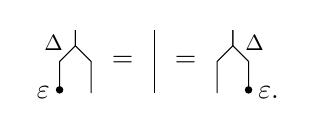
\begin{tikzpicture}[scale=.2]
\draw (-4,0)--(-4,2)--(-5,3)--(-5,4);
\draw (-6,0)--(-6,2)--(-5,3)--(-5,4);
\node [left, scale=.8] at (-5.3,3.2) {$\Delta$};
\draw [fill] (-6,.2) circle [radius=.2];
\node [left] at (-6,0) {$\varepsilon$};

\node at (-2,2) {=};
\draw (0,0)--(0,4);
\node at (2,2) {=};

\draw (4,0)--(4,2)--(5,3)--(5,4);
\draw (6,0)--(6,2)--(5,3)--(5,4);
\node [right, scale=.8] at (5.3,3.2) {$\Delta$};
\draw [fill] (6,.2) circle [radius=.2];
\node [right] at (6,0) {$\varepsilon$.};
\end{tikzpicture}
\end{equation*}
Notice that for any chain complex $C$, operad morphisms from $\Uleft(\A)$ to $\End_C$ correspond to counital coalgebra structures on $C$.

Let $W^{(1)}$ be the chain complex of free $\Z[\S_2]$-modules
\begin{equation*}
\begin{tikzcd}
\Z[\S_2]\{\nu\} &[0pt] \arrow[l, "1-T"'] \Z[\S_2]\{\mu\},
\end{tikzcd} 
\end{equation*}
which is isomorphic to the cellular chains on the standard model of the circle
\begin{equation*}
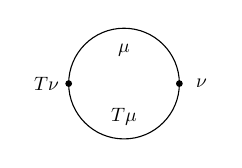
\begin{tikzpicture}
\draw (0,0) circle (20pt);
\node[scale=.7] at (0,12pt){$\mu$};
\node[scale=.7] at (0,-12pt){$T \mu$};
\node[scale=.7] at (-28pt,0){$T \nu$};
\node[scale=.7] at (28pt,0){$\nu$};
\draw [fill] (-20pt,0) circle [radius=1pt];
\draw [fill] (20pt,0) circle [radius=1pt];
\end{tikzpicture}
\end{equation*}
and let $W^{(0)}$ be the subcomplex generated by $\nu$. We think of $W^{(1)}$ as an $\S_2$-equivariant 1-cell with boundary $W^{(0)}$.

We regard these complexes as $\S$-bimodules concentrated in biarity $(2,1)$, and let $\varphi \colon W^{(0)} \to \A$ be define by sending $T \nu$ and $\nu$ respectively to
\begin{equation*}
	\begin{tikzpicture}[scale=.2]
	\draw (-4,0)--(-4,4);
	\draw (-6,0)--(-6,4);
	\draw [fill] (-6,.2) circle [radius=.2];
	\node [left] at (-6,0) {$\varepsilon$};
	
	\node at (0,.4) {and};
	
	\draw (4,0)--(4,4);
	\draw (6,0)--(6,4);
	\draw [fill] (6,.2) circle [radius=.2];
	\node [right] at (6,0) {$\varepsilon$.};
	\end{tikzpicture}
\end{equation*}
Consider the push-out
\begin{equation*}
\begin{tikzcd}
F(W^{(0)}) \arrow[r, "F(\varphi)"] \arrow[d] & \A \arrow[d, dashed] \\
F(W^{(1)}) \arrow[r, dashed] & \mu \vee \A
\end{tikzcd}
\end{equation*}
in the category of props. We think of $\mu \vee \mathcal A$ as the prop obtained by attaching a $1$-cell in biarity $(2,1)$ to $\A$.

Define $\M$ as the quotient of $\mu \vee \A$ by the ideal generated by
\begin{equation*}
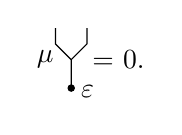
\begin{tikzpicture}[scale=.2]
\draw (5,4)--(5,3)--(6,2)--(6,0);
\draw (7,4)--(7,3)--(6,2);
\node [left] at (5.5,2) {$\mu$};
\draw [fill] (6,.2) circle [radius=.2];
\node [right] at (6,0) {$\varepsilon$};

\node at (9,2) {= 0.};
\end{tikzpicture}
\end{equation*}

We can give a more explicit description of $\M$ using the constructions of Subsection~\ref{ss:free props}.

The elements of $\M$ correspond to linear combinations of graphs obtained by grafting ...
\section{The cobar construction}

Let $R$ be a commutative ring. Given a graded $R$-module $M$ we denote by $s^{i}M$ the graded $R$-module given by $(s^{i}M)_n= M_{n-i}$.
Denote by $\textbf{dgAlg}_R$ the category of augmented differential graded associative $R$-algebras (dg algebras, for short) and by $\textbf{dgCoalg}_R$ the category of coaugmented differential graded coassociative $R$-coalgebras (dg coalgebras, for short). We recall the definition of the cobar functor 
$$\mathbf{\Omega}: \textbf{dgCoalg}_R \to \textbf{dgAlg}_R.$$

For any $(C, \partial, \Delta, \nu)  \in \textbf{dgCoalg}_R$ define
$$\mathbf{\Omega}(C, \partial, \Delta, \nu) := ( T(s^{-1}  \widetilde{C} ), D, \mu, \eta) \in \textbf{dgAlg}_R$$ where 
\begin{itemize}
\item $\widetilde{C}=\text{coker}(\nu: R \to C)$
\item $T(s^{-1} \widetilde{C})= R \oplus \widetilde{C} \oplus (\widetilde{C}  \otimes \widetilde{C} ) \oplus ( \widetilde{C} \otimes \widetilde{C} \otimes \widetilde{C} ) \oplus\cdots $
\item $\mu: T(s^{-1}  \widetilde{C} )^{\otimes 2} \to T(s^{-1}  \widetilde{C} ) $ is the free associative product given by concatenation of monomials
\item $D: T(s^{-1}  \widetilde{C} ) \to T(s^{-1}  \widetilde{C} )$ is the derivation of degree $-1$ determined by the linear map $$- s^{-1} \circ \partial \circ s^{+1} + (s^{-1} \otimes s^{-1}) \circ \Delta \circ s^{+1}: s^{-1}\widetilde{C} \to s^{-1}\widetilde{C} \oplus (s^{-1}\widetilde{C} \otimes s^{-1}\widetilde{C}) \hookrightarrow T(s^{-1}C)$$  by the graded Leibniz rule, and
\item $\eta: T(s^{-1}C) \to R$ is the augmentation map given by the natural projection map
\end{itemize}

The coassociativity of $\Delta$, the compatibility of $\partial$ and $\Delta$, and the fact that $\partial^2 =0$ together imply that $D^2=0$. This construction is clearly functorial with respect to maps in $\textbf{dgCoalg}_R$. We will denote $C=(C, \partial, \Delta, \nu)$ and $\mathbf{\Omega} (C, \partial, \Delta, \nu)$ simply by $\mathbf{\Omega}(C)$. 

In this article we will be concerned with \textit{connected} dg coalgebras, namely $(C, \partial, \Delta, \nu) \in \textbf{dgCoalg}_R$ which are non-negatively graded and $\nu: R \to C_0$ defines an isomorphism of coalgebras. We denote the category of connected dg coalgebras by $\textbf{dgCoalg}^0_R$. If $C \in \textbf{dgCoalg}_R^0$ then $\mathbf{\Omega}(C)$ is a dg algebra concentrated on non-negative degrees. 

The cobar construction was originally applied by Adams' to the dg coalgebra of normalized chains on a $1$-reduced simplicial set to obtain a dg algebra model for the chains on the based loop space \cite{Adams}. The cobar construction as a model for the based loop space was furthered studied in \cite{Baues} and more recently, in the non-simply connected setting in \cite{Hess-Tonks}, \cite{Rivera-Zeinalian}.


--- Recall the construction of a coassociative associative bialgebra on the cobar construction of an $E_2$-coalgebra following Kadeishvhili/Matthias Franz. In fact, I think we can do this in the context of $U(M)$-coalgebras? Namely, if start with a $U(M)$-coalgebra then we may construct a coassociative coproduct on the cobar construction on the underlying $A_{\infty}$-coalgera by looking at its $E_2$ part.

Discuss the localized version of the cobar construction. ---
\section{A necklical model for the based loop space}

Construct a functor from simplicial sets to monoidal necklical sets modelling the based loop space functor. 

Discuss relationship with the cobar construction on the chains on a simplicial set. 

\section{Main theorem and applications}

Adams ...
\begin{equation*}
\begin{tikzcd}
& \Mon_{\Ch} \\
\sSet^1 \arrow[ru] \arrow[r, "\chains"] & \coAlg \arrow[u, "\cobar"]
\end{tikzcd}
\end{equation*}

Modeling the loop space. Category of $1$-reduced simplicial sets.

Baues lifted this construction through the forgetful functor $\coAlg \to \Ch$ to the category of coalgebras using a cubical monoid.

\begin{equation*}
\begin{tikzcd}
\Mon_{\cSet} \arrow[r, "\chains"] & \Mon_{\coAlg_R} \\
\sSet^0 \arrow[r, "\chains"] \arrow[u, "\gcobar"] & \coAlg_R \arrow[u, "\cobar"]
\end{tikzcd}
\end{equation*}

The algebraic structure on the simplicial chains responsible for the Baues diagonal on $\Omega \chains$ is referred to as a homotopy $G$-coalgebra, which corresponds to the $E_2$-structure on simplicial chains, naturally an $E_\infty$-coalgebra.
Later, Kadeishvili \cite{Kadeishvili03cup-i} extended this construction to produce cup-$i$ coproducts on the cobar construction. 
The simplicial chains carry the structure of a coalgebra over the surjection operad, and Fresse \cite{Fresse03construction} constructed on the cobar construction of a surjection coalgebra the structure of a Barratt-Eccles coalgebra.
Our result is most similar to Fresse's.
As it will become clear, two key differences are that he uses distinct operads for chains and their cobar construction and does not relate his construction to cubical cochains, a hallmark of Baues's insight.


%Applications: if the natural chain map between the normalized chains on a cubical set and its triangulation preserves the $U(M)$-coalgebra structure (check?) we may deduce that our model is equivalent as a $E_{\infty}$-bialgebra to the normalized chains on the classical Kan loop group functor (this would use recent work of Rivera, Zeinalian, and Minichello).


Us

\begin{equation*}
\begin{tikzcd}
\Mon_{\cSet} \arrow[r, "\chains"] & \Mon_{\coAlg_{U(\M)}} \\
\sSet^0 \arrow[r, "\chains"] \arrow[u, "\gcobar"] & \coAlg_{U(\M)} \arrow[u, "\cobar"]
\end{tikzcd}
\end{equation*} 

\bibliographystyle{alpha} % ieeetr
\bibliography{biblio}

\end{document}